\documentclass[polish, twoside, 12pt]{mwart}
\usepackage[polish]{babel}
\usepackage{polski}
\usepackage[T1]{fontenc}
\usepackage[utf8]{inputenc}

\usepackage{hyperref}
\hypersetup{
    colorlinks,
    citecolor=black,
    filecolor=black,
    linkcolor=black,
    urlcolor=black
}
\usepackage{listings}

\usepackage{tabularx}
\usepackage{ltablex}
\newcolumntype{x}{p{4cm}}

\usepackage{tikz-qtree}

\usepackage{amsmath}

\usepackage{graphicx}
\graphicspath{ {../figures/} }

\let\stdsection\section
\renewcommand*{\section}{\clearpage\stdsection}
\emergencystretch=3em
\linespread{1.1}

\author{Kewin Polok}
\title{Praca dyplomowa magisterska}

\begin{document}

\maketitle
 
\newpage

\tableofcontents

\newpage

\listoffigures
 
\listoftables

\newpage

\section{Wstęp}

\subsection{Cel pracy}

\subsection{Układ pracy}

\section{Specyfikacja problemu}

\subsection{Założenia dotyczące problemu}

\section{Przeglądarka internetowa}

Przeglądarka internetowa (ang. \emph{web browser}) to program komputerowy służący do pobierania i wyświetlania stron internetowych udostępnianych przez serwery WWW. Komunikacja z serwerem odbywa się najczęściej za pomocą protokołu HTTP (ang. \emph{Hypertext Transfer Protocol})lub odpowiednika w wersji szyfrowanej HTTPS (ang. \emph{Hypertext Transfer Protocol Secure}). Nierzadko przeglądarki internetowe są w stanie obsługiwać inne protokoły takie jak np. FTP (ang. \emph{File Transfer Protocol}) wykorzystywany do serwerów plików, czy też protokoły POP3 (ang. \emph{Post Office Protocol}), IMAP (ang. \emph{Internet Message Access Protocol}) i SMTP (ang. \emph{Simple Mail Transfer Protocol}) wykorzystywane do poczty elektronicznej. 

\begin{figure}[ht]
  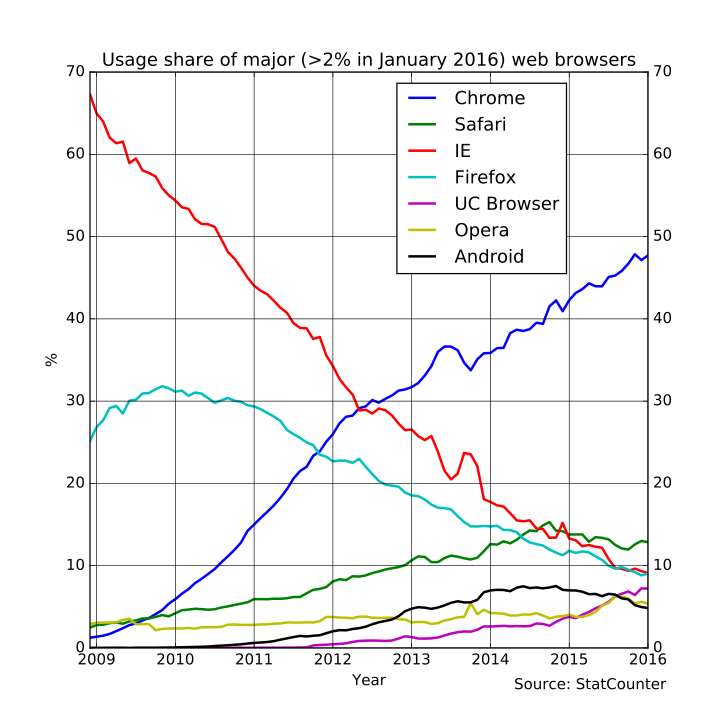
\includegraphics[width=\textwidth]{web-browers-usage-share.png}
	\caption{Udział najwaznieższych przeglądarek na rynku w latach 2009-2016}
\end{figure}

\subsection{Technologie}

Współczesne strony internetowe to nierzadko bardzo skompliowane aplikacje, dlatego też przeglądarki internetowe muszą bardzo dobrze obsługiwać wiele technologii, które działając razem pozwalają dostarczyć bardzo wysokiej jakości doświadczenia użytkownika (ang. \emph{User experience}). 

\subsubsection{HTML 5.1} \label{html}

Hipertekstowy język znaczników (ang. \emph{HyperText Markup Language}) to język służący do określenia struktury strony internetowej. Definicję HTML 5.1 stanowi W3C REC-HTML51 \cite{w3c-rec-html51}. Oprócz głównego tekstu HTML zawiera tak zwane znaczniki, które zawierają dodatkowe informacje pozwalające przeglądarce internetowej odpowiednio zinterpretować określony fragment strony interetowej. Za pomocą znaczników możemy formować fragmenty strony w takie struktury jak hiperłącza, akapity, listy, nagłówki, czy też formularze. Znaczniki najczęściej występują w parach (jako znacznik otwierając oraz zamykający) definiując zakres działania.

\lstinputlisting[language=HTML, caption=Przykładowa prosta strona internetowa z formularzem]{../examples/html.html}

Strona internetowa zaczyna się od \emph{<!DOCTYPE html>}. Jest to specjalny znacznik, który musi być umieszczony jako pierwszy. Informuje on przeglądarkę o tym, że tekst jest w formacie HTML. Kolejnym znacznikiem jest \emph{html} z atrybutem \emph{lang}, jest to główny znacznik, będacy korzeniem całej zagnieżdzonej struktury. Dodatkowo informuje o. Bardzo ważny, wyraźnie odseparowany fragment to znacznik \emph{head} zawierający infomację o systemie kodowania (w tym wypadku jest to  kodowanie UTF-8) oraz tytuł strony. Może on zawierać dodatkowe metadane opisujące stronę internetową. Z punktu widzenia użytkownika najważniejszym fragmentem jest znacznik \emph{body}, który zawiera właściwą treść, czyli w tym wypadku jest to głównie formularz \emph{form}. Dwa najważniejsze atrybuty opisujące formularz to \emph{action} informujący przeglądarkę gdzie wysłać dane wpisane przez użytkownika oraz \emph{method} na podstawie, którego przeglądarka wie jaką metodę protokołu HTTP zastosować. Przykładowy formularz zawiera jedno pole tekstowe \emph{input type="text"} oraz jedno pole do wpisywania haseł \emph{input type="password"}. Hasło wpisane w tego typu pole jest domyślnie ukryte przez przeglądarkę dla celów bezpieczeństwa. Oba pola dodatkowo opisane są etykietami \emph{label}. Ostatnim nieopisanym jeszcze znacznikiem jest \emph{button type="submit"}, który jest po prostu przyciskiem służącym do wysłania formularza. Każda przeglądarka posiada wbudowany zestaw styli, który definiuje wygląd każdego znacznika przewidzianego w dokumentacji HTML 5.

\begin{figure}[ht]
  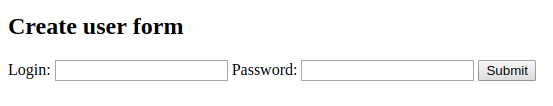
\includegraphics[width=\textwidth]{html-chrome.png}
	\caption{Przykład wyrenderowany w przeglądarce Chrome}
\end{figure}

\subsubsection{CSS 3}

Kaskadowe arkusze stylów (ang. \emph{Cascading Style Sheets}) to język służący do opisu wyświetlania struktury opisanej w języku HTML. Wersja 3 składa się z wielu modułów. Każdy z nich dodaje nowe możliwości lub rozszerza te zdefiniowane w CSS 2 zachowując wsteczną kompatybilność (ang. \emph{backward compatibility}).

\begin{enumerate}
  \item css3-background - specyfikacja W3C REC-CSS3-Background \cite{w3c-rec-css3-background}
  \item css3-box - specyfikacja W3C REC-CSS3-Box \cite{w3c-rec-css3-box}
  \item css-cascade-3 - specyfikacja W3C REC-CSS-Cascade-3 \cite{w3c-rec-css3-cascade}
  \item css3-color - specyfikacja W3C REC-CSS3-Color \cite{w3c-rec-css3-color}
  \item css3-content - specyfikacja W3C REC-CSS-Content-3 \cite{w3c-rec-css3-content}
  \item css-fonts-3 - specyfikacja W3C REC-CSS-Fonts-3 \cite{w3c-rec-css3-fonts}
  \item css3-gcpm - specyfikacja W3C REC-CSS-GCPM-3 \cite{w3c-rec-css3-gcpm}
  \item css3-layout - specyfikacja W3C REC-CSS-Template-3 \cite{w3c-rec-css3-template}
  \item css3-mediaqueries - specyfikacja W3C REC-CSS3-Mediaqueries \cite{w3c-rec-css3-mediaqueries}
  \item css3-multicol - specyfikacja W3C REC-CSS3-Multicol \cite{w3c-rec-css3-multicol}
  \item css3-page - specyfikacja W3C REC-CSS3-Page \cite{w3c-rec-css3-page}
  \item css3-selectors - specyfikacja W3C REC-CSS3-Selectors \cite{w3c-rec-css3-selectors}
  \item css-3-ui - W3C REC-CSS-UI-3 \cite{w3c-rec-css3-ui}
\end{enumerate}

Za pomocą CSS opisać można wszystkie pojęcia odpowiedzialne za reprezentację elementów HTML, takie jak rodzina czcionek, kolor tekstu, marginesy, czy też pozycja danego elementu względem innych elementów lub okna przeglądarki.

CSS został stworzony w celu odseparowania struktury dokumentu od formy jego prezentacji. Zalety tej separacji to zwiększony zakres dostępności witryny, zmniejszona zawiłość dokumentu, łatwiejsze wprowadzanie zmian w strukturze dokumentu. CSS ułatwia także zmiany w wyświetlaniu strony w zależności od obsługiwanego medium (ekran komputera, ekran tabletu, ekran telefonu komórkowego).

Arkusz stylów składa się z reguł określających styl dla wybranych elementów dokumentu. Reguła składa się z selektora oraz deklaracji. Selektor określa grupę elementów, którego ma dotyczyć deklaracja. Deklaracja określa formatowanie i składa się z nazwy jednej z właściwości i jej wartości napisanej po dwukropku. Deklaracja musi być otoczona nawiasami klamrowymi.

\begin{lstlisting}
selektor { 
	wlasciwosc: wartosc; 
}
\end{lstlisting}

Selektory oraz deklaracje można grupować. Zgrupowane selektory rozdziela się przecinkami, natomiast deklaracje średnikami.

\begin{lstlisting}
selektor, selektor2 { 
	wlasciwosc1: wartosc1;
	wlasciwosc2: wartosc2;
}
\end{lstlisting}

Selektory mogą poszukiwać elementy na podstawie wielu różnych wartośći, jedne z nich to:

\begin{itemize}
  \item nazwa elementu np. \emph{h1}
  \item atrybut \emph{class} elementu np. \emph{.my-class}
  \item identyfikator elementu, czyli atrybut \emph{id} np. \emph{\#element-id}
  \item połączenie wcześniejszych selektorów operatorem logicznym \emph{OR} np. \emph{h1.my-class}
  \item połączenie wcześniejszych selektorów operatorem logicznym \emph{AND} np. \emph{\#element-id .my-class}
\end{itemize}

Dobrą praktyką jest definiowanie selektorów na podstawie atrubutu \emph{class}, natomiast identyfikator, czyli atrybut \emph{id} powinien służyć do jednoznacznej identyfikacji elementu w strukturze HTML. Zgodnie z dokumentacją wiele znaczników może posiadać taką samą klasę, natomiast identyfikator aby spełniał swoje zadanie musi być unikalny.

Ponieważ standardowy wygląd znaczników z punktu widzenia użytkownika może być interpretowany jako bardzo prosty to współcześnie nieostylowane strony internetowe zdarzają się bardzo rzadko. W celu pokazania jak duża może być różnica pomiędzy standardowym, a specjalnie ostylowanym wyglądem strony internetowej przedstawiony zostanie poprzedni przykład strony z formularzem wzbogacony o bardzo lekką bibliotekę CSS o nazwie Milligram\cite{milligram}, której rozmiar wynosi tylko 2kb.

\begin{figure}[ht]
  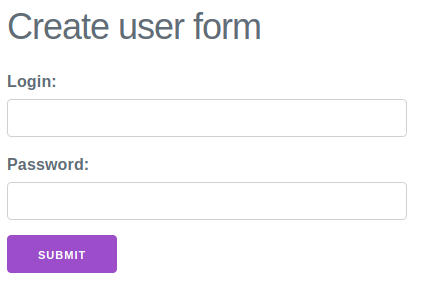
\includegraphics[width=\textwidth]{html-css-chrome.png}
	\caption{Ostylowany przykład wyrenderowany w przeglądarce Chrome}
\end{figure}

\subsubsection{JavaScript}

JavaScript to skryptowy język programowania, stworzony przez firmę Netscape, najczęściej stosowany na stronach internetowych. Pod koniec lat 90. XX wieku organizacja ECMA wydała na podstawie JavaScriptu standard języka skryptowego o nazwie ECMAScript. Najnowsza stabilna wersja ECMAScript nosi nazwę ECMAScript 2016 \cite{es2016} i została wydana 17 czerwca 2016. Organizacja ECMA zapowiedziała, że stabilna wersja tego standardu od wersji 2015 będzie ogłaszana co rok i to właśnie rok wydania będzie jednoznaczny z numerem wersji. Wcześniej mowa była o edycji standardu ECMAScript i do teraz często można się spotkać z zamiennem stosowaniem nazw ECMAScript 6 i ECMAScript 2015 (skracanych odpowiednio do ES6 i ES2015).

Najczęściej spotykanym zastosowaniem języka JavaScript są strony WWW. Skrypty napisane w tym języku najczęściej służą do zapewnienia interaktywności poprzez odpowiednie reagowanie na zdarzenia generowane przez użytkownika. Skrypty JavaScriptu uruchamiane przez strony internetowe mają znacznie ograniczony dostęp do komputera użytkownika. 

Platformy programistyczne, które zostaną zbadane w ramach pracy magisterskiej napisane są języku JavaScript. Wspomagają one proces pisania aplikacji internetowej dostarczając odpowiednich funkcji i organizująć strukturę strony internetowej zgodnie z wytycznymi konkretnej platformy programistycznej.

W języku HTML za umieszczanie skryptów JavaScript odpowiedzialny jest znacznik \emph{script} z opcjonalnymi parametrami \emph{type="text/javascript"} i \emph{language="javascript"}.

JavaScript może zostać użyty również po stronie serwera dzięki darmowemu środowisku uruchomieniowemu Node.js\cite{node.js}. Node.js zaprojektowany został do tworzenia wysoce skalowalnych aplikacji internetowych, szczególnie właśnie serwerów napisanych w języku JavaScript. Architektura Node.js składa się z silnika V8 \cite{v8} stworzonego przez Google i opiera się na sterowaniu zdarzeniami wykorzystującymi asynchroniczny system wejścia-wyjścia. Kod źródłowy jest otwarty (ang. \emph{open source}) i każdy może brać udział w jego rozwijaniu. Domyślnym menedżer pakietów dla Node.js jest Npm \cite{npm}, jednak warto zapoznać się z alternatywnym mendedżerem o nazwie Yarn \cite{yarn}, którego głównymi zaletami są szybsze pobieranie zależności oraz bardziej płaska stuktura drzewa pobranych zależności.

\subsubsection{DOM} \label{dom}

Obiektowy model dokumentu (ang. \emph{Document Object Model}) to zespół klas i interfejsów programistycznych umożliwiających dostęp do elementów strony napisanej w języku HTML. Istnieje kilka tzw. poziomów DOM (ang. \emph{level}):

\begin{enumerate}
  \item DOM Level 0 - nie stanowi oficjalnego standardu W3C \cite{w3c}, pierwotnie był modelem zaimplementowanym w przeglądarce Netscape Navigator 3.0, obecnie wspierają go wszystkie przeglądarki
  \item DOM Level 1 - specyfikacja W3C REC-DOM-Level-1 \cite{w3c-rec-dom-level-1} 
  \item DOM Level 2 - specyfikacja W3C REC-DOM-Level-2 \cite{w3c-rec-dom-level-2} 
  \item DOM Level 3 - definicję stanowi sześć specyfikacji
  \begin{itemize}
    \item DOM Level 3 Core - specyfikacja W3C DOM-Level-3-Core \cite{w3c-rec-dom-level-3-core}
    \item DOM Level 3 Load and Save - specyfikacja W3C DOM-Level-3-LS \cite{w3c-rec-dom-level-3-ls}
    \item DOM Level 3 XPath - specyfikacja W3C DOM-Level-3-XPath \cite{w3c-rec-dom-level-3-xpath}
    \item DOM Level 3 Views and Formatting - specyfikacja W3C DOM-Level-3-Views \cite{w3c-rec-dom-level-3-views}
    \item DOM Level 3 Requirements - specyfikacja W3C DOM-Level-3-Requirements \cite{w3c-rec-dom-level-3-requirements}
    \item DOM Level 3 Validation - specyfikacja W3C DOM-Level-3-Val \cite{w3c-rec-dom-level-3-val}
  \end{itemize}
\end{enumerate}

DOM pozwala dokonywać dowolnych modyfikacji poprzez tworzenie, usuwanie i modyfikację tzw. węzłów (ang. \emph{nodes}). Początkowo nie istniał standardowy obiektowy model dokumentu. Twórcy najpopulaniejszych przeglądarek tworzyłi własne niezgodne ze sobą modele. Organizacja W3C \cite{w3c} przygotowała ujednolicony standard obiektowego modelu dokumentu, w którym dokment jest dostępny pod postacią globalnego obiektu \emph{document}, który posiada metody do np. pobierania elementu na podstawie identyfikatora \emph{document.getElementById} lub na podstawie klasy \emph{document.getElementByClassName}. Standard W3C definiuje interfejsy DOM tylko dla języków JavaScript i Java.

\begin{figure}
  \centering
  \begin{tikzpicture}
    \Tree[.html 
      [.head 
        [.meta ]
        [.title ]
      ]
      [.body 
        [.h2 ]
        [.form 
            [.label ]
            [.input ]
            [.label ]
            [.input ]
            [.button ]
        ]
      ]
    ]
  \end{tikzpicture}
  \caption{Drzewo DOM wygenerowane dla przykładu opisanego w rozdziale \ref{html}}
\end{figure}

\subsubsection{CSSOM} \label{cssom}

Obiektowy model kaskadowych arkuszy stylów (ang. \emph{CSS Object Model}) to zespoł interfejsów programistycznych umożliwiających dostęp do stylów napisanych w języku CSS.

CSSOM blokuje wszystko przed wyświetleniem tzn. przeglądarka internetowa nie zacznie niczego renderować dopóki w pełni nie zostanie zakończona budowa CSSOM. W przypadku nieoptymalnej struktury CSS budowa może trwać bardzo długo co skutkuje widoczną dla użytkownika białą stroną bez zawartości.

CSSOM musi być zbudowany na nowo z każdym przeładowaniem strony, oznacza to, iż nawet jeśli pliki CSS zostały umieszczone w pamięci podręcznej (ang. \emph{cache}) to nie uchroni to przeglądarki przed koniecznością budowy CSSOM.

Istnieje związek pomiędzy kaskadowymi arkuszami stylów, które przeglądarka ładuje i skryptami JavaScript umieszczonymi na stronie. Żeby przeglądarka wyświetliła cokolwiek musi poprawnie zakończyć budowę CSSOM, w przypadku gdy budowa ta zostanie wstrzymana przez skrypty czas potrzebny na wyświetlenie jakiegokolwiek elementu wzrośnie. W przypadku nieoptymalnej kombinacji skryptów oraz stylów czas ten może wzrosnąc drastycznie skutkując bardzo negatywnymi doświadczeniami użytkownika, w najgorszym wypadku spowodować zniechęcenie użytkownika do dalszego oczekiwania i opuszczenie strony.

\begin{figure}
  \centering
  \resizebox{\textwidth}{!}{
    \begin{tikzpicture}
      \Tree[.body(font-size:10px) 
        [.h1(font-size:1.6rem) ]
        [.form(font-size:1.4rem) 
          [.label(font-size:1.2rem) ]
          [.input(font-size:1.2rem) ]
        ]
        [.button(font-size:1.4rem) ]
      ]
    \end{tikzpicture}
  }
  \caption{Przykładowe drzewo CSSOM wygenerowane dla przykładu opisanego w rozdziale \ref{html}}
\end{figure}
\subsubsection{HTTP/1.1} \label{http/1.1}

Protokół przesyłania dokumentów hipertekstowych (ang.\emph{(Hypertext Transfer Protocol)}) to protokół za pomocą którego przysła się żadania udostępnienia dokumentów z serwera WWW oraz informacje z forumlarzy internetowych. Obecną definicję HTTP stanowi RFC 2616 \cite{rfc2616}

Protokół HTTP udostępnia znormalizowany sposób komunikowania się komputerów ze sobą. Określa on formę żądań (ang. \emph{requests}) klienta dotyczących danych oraz formę odpowiedzi (ang. \emph{responses}) serwera na te żądania. Klientem może być np. przeglądarka internetowa. Jest zaliczany do protokołów bezstanowych (ang. \emph{stateless}) ponieważ nie zachowuje żadnych informacji o poprzednich transakcjach z klientem. Pozwala to znacznie zmniejszyć obciążenie serwera, jednak uniemożliwia zapamiętanie konkretnego stanu użytkownika w sytuacji gdy jest to potrzbne np. przy implementacji koszyka z zakupami w sklepie internetowym. Najczęstszym rozwiązaniem tego problemu jest wprowadzenie mechanizmu ciasteczek (ang. \emph{cookies}). Ciasteczka to mały fragment tekstu zawierający pary klucz-wartość. Przesyłane są one z każdym żądaniem do serwera. Alternatywne rozwiązania to ukryte parametry (gdy aktualna strona zawiera formularz) oraz parametry umieszczone w ujednoliconym formacie adresowania zasobów (ang. \emph{Uniform Resource Locator}.

Wywołania protokołu HTTP zaczynają się od \url{http://}. HTTP standardowo korzysta z portu numer 80 protokołu kontroli transmisji (ang. \emph{Transmission Control Protocol}).

Zapytanie HTTP zaczynaja się od nazwy metody, która określa akcję jaką obiekt tworzący zapytanie chce wykonać na zasobie podstępnym pod określonym adresem. Dostępne metody to:

\begin{enumerate}
  \item \emph{GET} - pobranie zasobu
  \item \emph{HEAD} - pobranie informacji o zasobie, metoda stosowana do sprawdzania dostępności zasobu
  \item \emph{PUT} - aktualizacja zasobu
  \item \emph{POST} - stworzenie nowego zasobu
  \item \emph{DELETE} - usunięcie zasobu
  \item \emph{OPTIONS} - pobranie informacji o możliwych operacjach do wykonania na zasobie
  \item \emph{TRACE} - metoda stosowana do diagnostyki kanału komunikacyjnego
  \item \emph{PATCH} - częściowa aktualizacja zasobu
\end{enumerate}

Poniżej przedstawione przykładowe żądanie HTTP/1.1 przeglądarki Chrome i odpowiedź serwera opisanego w rozdziale \ref{server}.

\begin{lstlisting}[caption=Przykładowe żądanie HTTP/1.1,]
GET / HTTP/1.1
Host: localhost:8080
Connection: keep-alive
Pragma: no-cache
Cache-Control: no-cache
Upgrade-Insecure-Requests: 1
User-Agent: Mozilla/5.0 (X11; Linux x86_64) AppleWebKit/537.36 
  (KHTML, like Gecko) Chrome/60.0.3112.90 Safari/537.36
Accept: text/html,application/xhtml+xml,application/xml;q=0.9,
  image/webp,image/apng,*/*;q=0.8
Accept-Encoding: gzip, deflate, br
Accept-Language: pl-PL,pl;q=0.8,en-US;q=0.6,en;q=0.4
\end{lstlisting}

\begin{lstlisting}[caption=Przykładowa odpowiedź HTTP/1.1]
HTTP/1.1 200 OK
X-Powered-By: Express
Content-Type: text/html; charset=utf-8
Content-Length: 116
ETag: W/"74-IGpXmXtcB0E/yn+QbK3UFXMrMU8"
Date: Tue, 15 Aug 2017 10:28:41 GMT
Connection: keep-alive
\end{lstlisting}

\subsubsection{HTTPS} \label{https}

Bezpieczny protokół przesyłania dokumentów hipertekstowych (ang. \emph{Hypertext Transfer Protocol Secure}) to szyfrowana wersja protokołu HTTP. Obecną definicję HTTPS stanowi RFC 2660 \cite{rfc2660}

W odróżnieniu od protokołu HTTPS protokół HTTP do komunikacji stosuje niezaszyfrowany tekst. HTTPS początkowo szyfrował dane za pomocą protokołu SSL (ang. \emph{Secure Socket Layer}), natomiast obecnie używany jest protokół TLS (ang. \emph{Transport Layer Security}). Szyfrowanie zapobiega przechtywywaniu i zmienianiu przesyłanych danych. 

Wywołania protokołu HTTPS zaczynają się od \url{https://}. HTTPS standardowo korzysta z portu numer 443 protokołu kontroli transmisji. 

\subsubsection{HTTP/2} \label{http/2}

Protokół HTTP/2 to unowocześniejszego protokołu HTTP/1.1. Został on opracowany na podstawie wczesnych wersji ekperymentalnego protokołu SPDY \cite{spdy}. Obecną definicję HTTP/2 stanowi RFC 7540 \cite{rfc7540}. W przeciwieństwie do wersji HTTP/1.1, protokół HTTP/2 jest w pełni binarny tzn. że tekst zrozumiały dla człowieka zastąpiony został zbiorem tak zwanych ramek (ang. \emph{frames}) o ściśle określonym formacie i zastosowaniu. Poniżej przedstawiono najważniejsze zalety protokołu HTTP/2.

\begin{enumerate}
  \item \emph{Multipleksowanie} - protokół nawiązuje tylko jedno trwałe połączenie z serwerem za pomocą którego pobierane są wszystkie pliku niezbędne do prawidłowego wyświetlenia strony
  \item \emph{Powiadomienia Push} - serwer może wysłać dodatkowe informacje np. może wysłać pliki, które są potrzebne do prawidłowego wyświetlenia strony zanim przeglądarka internetowa zauważy tą potrzebę
  \item \emph{Ustalanie priorytetów} - każde zapytanie o plik posiada swój priorytet, który nadawany jest przez serwer. Umożliwia to najpierw pobranie najważniejszych plików, które pozwolą wyrenderować kluczowe fragmenty strony internetowej, a następnie doczytać kolejne elementy
  \item \emph{Kompresja nagłówków} - protokół HTTP/2 unika duplikacji informacji występującyh pomiędzy różnymi nagłówkami i wysyła je w skompresowanym formacie
  \item \emph{Szyfrowanie} - pomimo, iż szyfrowanie według protokołu HTTP/2 nie jest wymagane to większość najważniejszych przeglądarek internetowych implementuje HTTP/2 wyłącznie z wykorzystaniem protokołu TLS
\end{enumerate}

\begin{figure}[ht]
  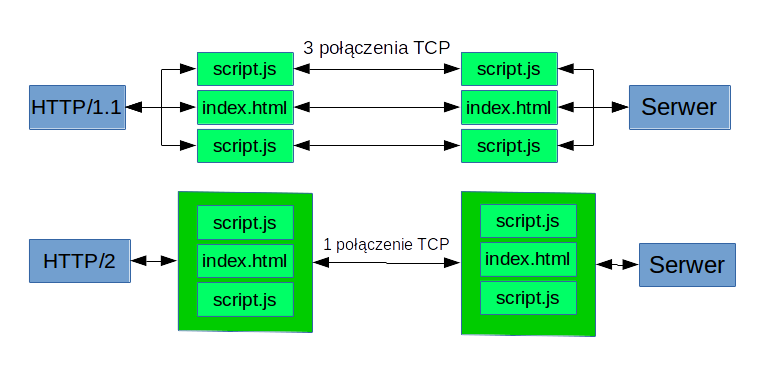
\includegraphics[width=\textwidth]{http2-mux.png}
	\caption{Multipeksowanie HTTP/2}
\end{figure}

\subsection{Proces wyświetlania strony internetowej}

Końcowym produktem przeglądarki internetowej jest w pełni załadowana i wyrenderowana strona internetowa, która oferuje użytkownikowi wszystkie zaimplementowane wcześniej funkcjonalności. Proces, który jest odpowiedzialny za dostarczenie tego produktu można podzielić na cztery etapy.

\begin{enumerate}
  \item pobieranie
  \item parsowanie
  \item budowanie
  \item renderowanie
\end{enumerate}

\subsubsection{Pobieranie}

Proces ładowania strony internetowej w przeglądarce zaczyna się od pobrania treści strony internetowej wraz ze wszystkimi zasobami potrzebnymi do jej wyświetlenia.
Przeglądarka pobiera wszystkie elementy za pomocą żądań \emph{HTTP}. Użytkownik może rozpocząć pobieranie na kilka sposbów:

\begin{enumerate}
  \item wpisanie adresu strony internetowej
  \item kliknięcie na odnośnik przekierowujący do innej strony lub do podstrony aktualnej strony internetowej
  \item przeładowanie aktualnej strony internetowej
\end{enumerate}

Moment stworzenia pierwszego żądania równoznaczny jest z początkiem wydarzenia które nosi nazwę "\emph{Navigation Start}". Zdarzenie to jest punktem, w którym przeglądarka zaczyna zbierać dodatkowe informacje na temat wydajności np. o czasie ładowania strony. Przeglądarka internetowa tworzy żądanie zgodnie z zasadami protokołu HTTP/1.1, który został bardziej szczegółowo opisny w rozdziale \ref{http/1.1}. Jeśli serwer wspiera obsługę nowszej wersji HTTP/2 wtedy wykorzystany jest nowszy protokół opisany w rozdziale \ref{http/2}. Całe wykonanie żądania przez przeglądarkę możemy podzielić na poszczególne fazy:

\begin{enumerate}
  \item \emph{Kolejkowanie} - przeglądarka kolejkuje żądania w następujących sytuacjach:
    \begin{itemize}
      \item aktualnie istnieją inne żądania do przetworzenia o wyższym priorytecie
      \item aktualnie istnieje już sześć otwartych połączen TCP dla konkretnego źródła (ang. \emph{origin}). Ograniczenie to dotyczy tylko HTTP/1.0 oraz HTTP/1.1
    \end{itemize}
  \item \emph{Odroczenie} - żądanie czeka na swoją kolej na przetworzenie z przyczyn wymienionych we wcześniejszym podpunkcie
  \item \emph{Podgląd DNS} - przeglądarka stara się przetłumaczyć adres internetowy na adres IP za pomocą usługi systemu nazw domenowych (ang. \emph{Domain Name System})
  \item \emph{Negocjowanie z pośrednikiem} - przeglądarka prowadzi negocjacje z serwerem pośredniczącym (ang. \emph{proxy})
  \item \emph{Wysłanie żądania} - przeglądarka wysyła żądanie do serwera
  \item \emph{Oczekiwanie} - przeglądarka oczekuje na pierwsze bajty odpowiedzi, w tym czasie mierzony jest parametr TTFB (ang. \emph{Time To First Byte}) oznaczający czas jaki minął zanim przeglądarka otrzymała pierwszy bajt odpowiedzi
  \item \emph{Pobieranie zawartości} - przeglądarka pobiera całą zawartość odpowiedzi
  \item \emph{Otrzymanie notyfikacji Push} - serwer wysyła dodatkowe dane dla przeglądarki, jest to element unikalny dla HTTP/2
  \item \emph{Czytanie notyfikacji Push} - przeglądarka czyta oraz interpretuje otrzymane wcześniej dodatkowe dane
\end{enumerate}

\begin{figure}[ht]
  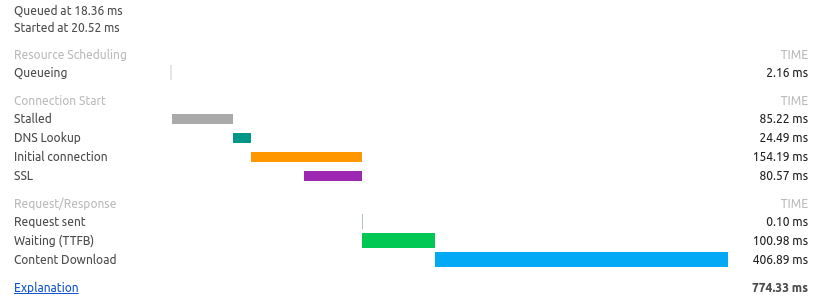
\includegraphics[width=\textwidth]{request-timing-chrome.png}
	\caption{Przykładowy widok przedstawiający czas trwania poszczególnych faz przetwarzania żądania wygenerowany za pomocą Chrome DevTools}
\end{figure}

\subsubsection{Parsowanie}

W momencie gdy przeglądarka w pełni przetworzy żądanie i otrzyma dokument w postaci pliku zawierającego kod HTML wtedy następuje proces czytania treści tego pliku w procesie zwanym parsowaniem. Pod pojęciem parsowanie ukrywa się czytanie treści z uwzględnieniem analizy składniowej specyficznej dla konkretnego języka. W przypadku języka HTML przeglądarka oczekuje poprawnie zdefiniowanych znaczników z właściwymi parametrami. 

Jeśli przeglądarka napotka znacznik odnoszący się do kolejnego zasobu wtedy proces parsowania zostaje zatrzymany i tworzone jest żądanie  w celu pobrania zawartości potrzebnej do pełnego wyświetlenia strony. Dopiero gdy przeglądarka pobierze cały zewnętrzny zasób proces parsowania zostaje kontynuowany. Znaczniki blokujące poprzez tworzenie odniesienia do zewnętrznego zasobu to:

\begin{enumerate}
  \item \emph{<link rel="stylesheet" type="text/css" href="style.css\">} - załączenie pliku ze stylami CSS
  \item \emph{<script type="text/javascript\" src="script.js\">} - załączenie pliku z kodem w języku JavaScript
  \item \emph{<img src="image.png\">} - załączenie pliku graficznego
\end{enumerate}

\subsubsection{Budowanie}

W chwili, w której przeglądarka zakończy parsowanie dokumentu i wszystkie zewnętrzne zasoby zostaną pobrane następuje proces budowania strony, czyli łączenia informacji znalezionych w głównym pliku HTML oraz pobranych zasobach. Na budowę strony składają się trzy kroki:

\begin{enumerate}
  \item \emph{Konstrukcja DOM} - obiektowa reprezentacja struktury opisanej w pliku HTML. Szerzej opisana w rozdziale \ref{dom}
  \item \emph{Konstrukcja CSSOM} - obiektowa reprezentacja kaskadowych arkuszy stylów. Szerzej opisana w rozdziale \ref{cssom}
  \item \emph{Konstrukcja drzewa renderowania (ang. Render Tree)} - drzewiasta struktura będąca połączeniem DOM oraz CSSOM, na podstawie którego przeglądarka jest w stanie poprawnie wyświetlić stronę internetową
\end{enumerate}

\subsubsection{Renderowanie}

Po wykonaniu wszystkich wcześniejszych kroków przeglądarka jest w końcu gotowa przejść do procesu renderowania. Większość współczesnych urządzeń odświeża ekran z częstotliwością 60 razy na sekundę. Jeśli aktualnie wykonywana jest jakaś animacja, przesuwanie lub użytkownik zwyczajnie przewija stronę internetową wtedy przeglądarka musi dopasować się do częstotliwości odświeżania urządzenia i przygotować nowy obrazek lub klatkę (ang. \emph{frame}) dla każdego pojedynczego odświeżenia ekranu. Każda z tych klatek posiada 16 milisekund na przygotowanie się do wyświetlenia. Wynika to z bardzo prostego obliczenia:

\begin{equation}
  \frac{1s}{60} = 16.66 ms
\end{equation}

Należy jednak pamiętać o tym, że przeglądarka posiada również swoje zadania do wykonania dlatego w rzewczywistości warto wykonać wszystkie własne zadania w czasie ponizej 10 milisekund. Po przekroczeniu tej wartości spada częstotliwość wyświetlania klatek co może objawiać się efektem migotania elementów wyświetlanych na ekranie. Migotanie jest niechcianym zjawiskiem ponieważ odbija się bardzo negatywnie na doświadczeniach użytkownika korzystającego ze strony internetowej.

Proces renderowania możemy podzielić na pięć postępujących po sobie etapów tzw. rurociągu (ang. \emph{pipeline}). Każdy z tych etapów ma znączacy wpływ na to w jaki sposób wyświetlone zostaną piksele na ekranie.

\begin{figure}[ht]
	\caption{Etapy rurociągu procesu renderowania}
\end{figure}

\begin{enumerate}
  \item \emph{JavaScript / CSS} - język \emph{JavaScript} ten może zostać użyty do zadań, które ostatecznie skutkują wizualnymi zwianami na ekranie. Do tego typu zadań możemy zaliczyć np. wywołanie animacji, sortowanie zestawu danych, dodawanie elementów do strony za pomocą interfejsów \emph{DOM}. Animacje mogą również być definiowane za pomocą kasakdowych arkuszy styli.
  \item \emph{Kalkulacja styli} - służy do określenia które reguły CSS zaaplikować do konkretnych elementów na podstawie pasujących selektorów oraz oblicza wartości poszczególnych właściwości \emph{CSS}
  \item \emph{Układ (ang. Layout)} - przeglądarka wie już co wyświetlić na podstawie \emph{DOM}, wie też w jaki sposób to wyświetlić na podstawie \emph{CSSOM} oraz zna relację pomiędzy tymi dwoma elementami na podstawie \emph{Render Tree}. Na tym etapie przeglądarka oblicza jak dużą przestrzeń elementy będą zajmować na ekranie. Obliczenia te są potrzebne ponieważ właściwości jednego elementu często wpływają relatywnie na inne. Przykładowo szerokość elementu \emph{body}, które umiejscowione jest bardzo wysoko blisko korzenia w drzewie elementów wpłynie na szerokość wszystkich podelementów aż do tzw. liści. Z racji dużej ilości obliczeń proces ten może mocno angażować procesor.
  \item \emph{Malowanie (ang. Paint)} - malowanie jest processem wypełniania poszczególnych pikseli na ekranie. Sprowadza się do wyświetlenia tekstu, kolorów, obrazków, obramowań, cieni, czyli głównie wszystkiego co wpływa na wizualną część każdego elementu. Najczęściej elementy malowane są na wielu powierzchniach popularnie nazywanych warstwami
  \item \emph{Kompozycja (ang. Compositing)} - ponieważ elementy strony mogły zostać potencjalnie namalowane na wielu różnych warstawach, przeglądarka musi wyświetlić warstwy w odpowiedniej kolejności. Dotyczy to szczególnie elementów, które wzajemnie na siebie nachodzą, od błędnej kompozycji może zależeć czy element, który powinien być przykryty przypadkowo zostanie wyrysowany na warstwie znajdującej się na samej górze
\end{enumerate}

Każda część rurociągu może potencjalnie wywołać efekt migotania dlatego też ważne jest dokładne zrozumienie jest co powoduje wyzwalanie poszczególnych części.

Czasami można spotkac się z określeniem rasteryzacji (ang. \emph{rasterization}) używanym jako synonim etapu malowania. Dzieję się tak dlatego ponieważ malowanie składa się z dwoch zadań:

\begin{enumerate}
  \item tworzenia listy prymitywnych elemtów do wyrysowania takich jak np. punkty, odcinki, krzywe, okręgi, koła, kwadraty
  \item wypełniania pikseli na ekranie
\end{enumerate}

To właśnie ostatnie z wymienionych zadań jest właściwą rasteryzacją, czyli działaniem polegającym na jak najwierniejszym przedstawieniu płaskiej figury geometrycznej na urządzeniu rastrowym, dysponującym skończoną rozdzielczością, w naszym przypadku na ekranie urządzenia. Warto przytoczyć tutaj fakt, iż niektóre implementacje wykonują wymienione zadania na różnych wątkach procesora (ang. \emph{threads}), jednak dzieje się to poza jakąkolwiek kontrolą programisty.

Przygotowanie klatki do wyświetenia nie zawsze musi przechodzić przez wszystkie pięc etapów rurociągu. Istnieją trzy kombinacje elementów, które odgrywają rolę przy przygotowaniu klatki w momencie gdy nastąpiła wizualna zmiana obojętnie czy z powodu kodu napisanego w języku \emph{JavaScript}, czy też z powodu zdefiniowanych styli \emph{CSS}.

\begin{enumerate}
  \item \emph{JavaScript / CSS > Style > Layout > Paint > Composite} - pełne przejście przez wszystkie etapy. Ma miejsce w momencie gdy zmeinia się właściwość powiązana z układem elementów na stronie np. szerokość, wysokośc, pozycja elementu. Przeglądarka musi sprawdzić wszystkie pozostałe elementy, dokonać odpowiednich obliczeń potrzebnych na pełne przemalowanie warstw, a ostatecznie dokonania ich kompozycji
  \item \emph{JavaScript / CSS > Style > Paint > Composite} - kombinacja ta ma miejsce w momencie gdy zmienia się właściwość powiązana wyłącznie z malowaniem strony jak np. tło, kolor tekstu. Przeglądarka nie musi wtedy na nowo opracowywać układu strony, co nie zmienia faktu, że musi przejść przez etap malowania
  \item \emph{JavaScript / CSS > Style > Composite} - najbardziej pożądana kombinacja ponieważ nie wymaga ani opracowania układu strony, ani jej przemalowania. Ma miejsce tylko gdy zmienia się właściwość nie powiązana ze wcześniej wymienionymi etapami
\end{enumerate}

\begin{figure}[ht]
	\caption{JavaScript / CSS > Style > Layout > Paint > Composite}
\end{figure}

\begin{figure}[ht]
	\caption{JavaScript / CSS > Style > Paint > Composite}
\end{figure}

\begin{figure}[ht]
	\caption{JavaScript / CSS > Style > Composite}
\end{figure}

\subsection{Model współbieżności oraz pętla zdarzeń}

Język JavaScript posiada model współbieżności oparty na pętli zdarzeń (ang. \emph{event loop}. Ten model różni się od modeli zaimplementowanych w innych językach jak np. \emph{C} lub \emph{Java}.

Poniższe sekcje wyjaśniają model teoretyczny. Nowoczesne silniki JavaScript implementują i optymalizują opisaną tutaj semantykę.

\begin{figure}[ht]
  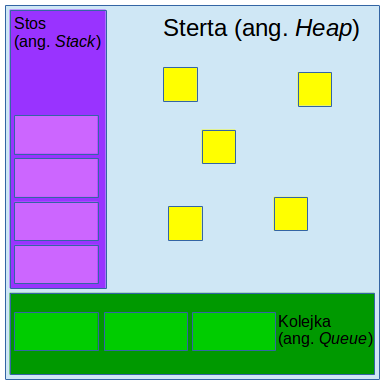
\includegraphics[width=\textwidth]{concurrency-model.png}
	\caption{Wizualizacja modelu}
\end{figure}

\subsubsection{Stos}

Wywołania funkcji tworzą ramki (ang. \emph{frames}), które odkładane są na strukturze danych o nazwie stos(ang. \emph{stack}).

\begin{lstlisting}
function foo(b) {
  var a = 1;
  return a + b;
}

function bar(x) {
  var y = 1;
  return foo(x * y);
}

console.log(bar(2));
\end{lstlisting}

Na przedstawionym przykładzie w momencie wywołania funkcji \emph{bar} zostaje utworzona pierwsza ramka przechowująca argumenty przekazane do tej funkcji oraz lokalne zmienne. Następnie gdy wewnątrz funkcji \emph{bar} wywoływana jest funkcja \emph{foo} tworzona jest druga ramka przechowująca te same informacje tj. przekazane argumenty oraz lokalne zmienne. Ramka umieszczana jest na samej górze stosu nad pierwszym elementem. Kiedy następuje powrót z funkcji \emph{foo} element na samej górze stosu zostaje zdjęty (pozostawijąc tylko ramkę powiązaną z wywołaniem funkcji \emph{bar}). Po powrocie z funkcji \emph{bar} stos powonie staje się pusty.

\subsubsection{Sterta}

Obiekty utworzone w języku JavaScript są umieszczane w stercie (ang. \emph{heap}). Poprzez stertę rozumi się duzą w większości nieustrukturyzowaną przestrzeń pamięci.

\subsubsection{Kolejka}

Środowisko wykonawcze języka JavaScript zawiera kolejkę (ang. \emph{queue}), która składa się z wiadomości do przetworzenia. Funkcja jest przypisana do odpowiedniej wiadomości. W momencie gdy stos posiada wystarczająco dużo miejsca wiadomość jest pobierana z kolejki i przetwarzana. Przetwarzanie polega na wywołaniu skojarzonej funkcji, a tym samym utworzeniu początkowej ramki stosu.
Przetwarzanie wiadomości kończy się, gdy stos staje się pusty.

\subsubsection{Pętla zdarzeń}

Pętla zdarzeń uzyskała swoją nazwę ze względu na to, jak zwykle jest to implementowana. Działanie pętli zdarzen obrazuje poniższy pseudokod:

\begin{lstlisting}
while (queue.waitForMessage()) {
  queue.processNextMessage();
}
\end{lstlisting}

Fragment \emph{queue.waitForMessage()} oczekuje synchronicznie, aż pojawi się wiadomość w kolejkce. Pętla zdarzen posiada kilka bardzo ważnych własności:

\begin{enumerate}
  \item \emph{Działanie do końca} - każda wiadomość jest przetwarzana całkowice przed przetworzeniem jakiejkolwiek innej wiadomości. To zachowanie gwarantuje, iż raz wywołana funkcja będzie działać do końca przed uruchomieniem dowolnego innego kodu. Jako przykład innego działania można przedstawić język C, gdzie np. jeśli funkcja dziąła w wątku może być zatrzymana w dowolnym momencie, aby uruchomić inny kod w innym wątku. Minusem tego modelu jest możliwość zaistnienia sytuacji w której przetwarzanie wiadomości trwa bardzo długo, w tym czasie aplikacja internetowa nie jest w stanie przetworzyć interakcji użytkownika. Przeglądarka obsługuje tą sytuację wyświetlając informację o tym, że wykonywanie skryptu trwa bardzo długo. Może to zniechęcić użytkownika do opuszczenia strony lub jej ponownego odświeżenia. Dobrą praktyką jest pisanie jak najkrótszej implementacji przetwarzania wiadomości
  \item \emph{Sposób dodawania wiadomości} - w przeglądarce internetowej wiadomości dodawane są do kolejki w dowolnym momencie, w którym zdarzenie to ma miejsce pod warunkiem, że została dodana funkcja nasłuchująca konkretnego wydarzenia. Bez nasłuchiwania zdarzenia wiadomość ulega przepadnięciu. Istnieje możliwość dodanie wiadomości do kolejki za pomocą funkcji \emph{setTimeout}. Wiadomość ta zostanie dodana do kolejki po upływie czasu podanego jako argument funkcji. W przypadku, w którym w kolejce nie ma innej wiadomości to nowo dodana wiadomość zostanie przetworzona od razu, jeśli istnieją jakieś inne, wtedy komunikat dodany metodą \emph{setTimeout} będzie musiał poczekać zanim nie zostaną one przetworzone. Z tego powodu argument podany jako czas wkazuje na minimalny czas, a nie na gwarantowany czas. Z tego powodu należy również mieć na uwadze fakt, iż wywołanie funkcji \emph{setTimeout} z opóżnieniem 0 milisekund nie spowoduje przetworzena wiadomości od razu. Wszystko zależy od aktualnego stopnia zapełnienia kolejki.
  \item \emph{Brak blokowania} - w przeciwieńswie do wielu innych języków JavaScript nigdy się nie blokuje. Obsługa wejścia / wyjścia zazwyczaj odbywa się za pośrednictwem zdarzeń i wywołan zwrotnych. Tym samym gdy aplikacja nadal może przetwarzać inne rzeczy jak np. wprowadzanie danych przez użytkownika
\end{enumerate}

\section{Biblioteki programistyczne do tworzenia aplikacji internetowych}

Aktualny wybór bibliotek programistycznych do tworzenia aplikacji internetowych w języku \emph{JavaScript} jest bardzo szeroki. Zdecydowana większość bibliotek tworzona i utrzymywana jest zgodnie z zasadami wolnego oprogramowania \emph{Open Source}. Im większa popularność biblioteki tym większa szansa na wkład użytkowników w postaci nowych funkcjonalności, poprawiania błędów (w tym tych związanych z bezpieczeństwem), czy też optymalizacji. Podjęcie decyzji jakiej biblioteki użyć może być bardzo trudne zwłaszcza, że dosłownie z miesiąca na miesiąć może powstać nowa biblioteka zaskarbiająca sobie dużą sympatię programistów i tym samem pociągnać za sobą przepływ społeczeństwa zaangażowanego w tworzenie oprogramowania. 

\subsection{Charakterystyczne cechy}

Współczesne biblioteki często wzajemnie zapożyczają i implementują pomysły, czy też rozwiązania, które sprawdziły się w środowisku produkcyjnym. Rozwiązania te pozwalają na szybkie tworzenie oprogramowania przez doświadczonego programistę, ale narzucona struktura oprogramowania jest na tyle prosta, że może nad nim pracować osoba mniej doświadczona programistycznie. Niektóre ze stosowanych roziązań niosą pozytywne efekty również dla użytkownika końcowego w postaci szybko renderującej się i reagującej na akcje użytkownika strony internetowej.

\subsubsection{Komponenty}

Architektura strony internetwoej zbudowanej za pomocą współczesnych bibliotek programistycznych opiera się najczęściej na idei komponentów. Poprzez komponenty rozumi się fragment strony internetowej, który posiada jasno określoną odpowiedzialność. Komponenty buduje się z połaczęnia HTML, JavaScript oraz CSS, tym samym komponent zawiera wszystkie informacje potrzebne do wyświetlenia oraz działania. Dzięki tej niezależności komponenty są w łatwy sposób testowalne, mają jasno określony interfejs za pomocą którego komunikują się z innymi komponentami. Raz określony komponent może być użyty w wielu miejscach co pozwala uniknąc niepotrzebnej duplikacji kodu.

Struktura strony internetowej opartej na komponentach może zostać przedstawiona za pomocą drzewa, którego korzeniem jest główny komponent, który najczęściej po prostu składa się z kilku komponentów o bardziej specyficznych odpowiedzialnościach. Te komponenty moga składać się z kolejnych i tak dalej. 

Komponenty mogą przechowywać swój aktualny stan potrzebny do poprawnego wyświetlenia oraz działania wykorzystując do tego zmienne o zakresie prywatnym to jest takim, który nie jest w żaden sposób udostępniany innym obiektom.

Kolejną charakterystyczną cechą komponentów jest ich cykl życia (ang. \emph{lifecycle}). Programista tworząc komponent może definiować fragmenty kodu, który zostanie uruchomiony w pewnych sytuacjach. Te sytuacje zależą od biblioteki ale najczęściej to moment w którym komponent zostaje stworzony, moment w którym zostaje niszczony oraz moment, w którym zmieniają się dostarczane do niego dane poprzez z góry określony interfejs.

\subsubsection{Wirtualny obiektowy model dokumentu}

Niektóre z bibliotek implementują mechanizm wirutalnego obiektowego modelu dokumentu (ang. \emph{ Virtual DOM}), jego głównym celem jest przyspieszenie działania aplikacji. Działanie tego mechanizmu polega na trzymaniu w pamięci kopii aktualnego obiektowego modelu dokumentu. W momencie, w którym DOM się zmienia np. w wyniku działania użytkownika najpierw modyfikowana jest wirtualna kopia przechowywana w pamięci. Po ustabilizowaniu się kopii wirtualnej zmiany nakładane są na rzeczywisty DOM.

Operacje wykonywane na kopii przechowywanej w pamięci są szybsze niż operowanie na rzeczywistym obiekcie. Dodatkowo liczba nakładanych zmian jest minimalna, oczekiwanie na stabilizację kopii pozwala uniknąć wprowadzania zmian, które są tymczasowe i nie mają miejsca w wersji finalnej.

\subsubsection{Wstrzykiwanie zależności}

Niektóre z bibliotek udostępmniają mechanizm wstrzykiwania zależności (ang. \emph {Dependency injection}), jest to jeden z możliwych sposobów dostarczania zależności do komponentów.

Ogólnie rzecz biorąc wstrzykiwanie zależności to wzorzec projektowy i wzorzec architektury oprogramowania polegający na usuwaniu bezpośrednich zależności pomiędzy komponentami. Polega na przekazywaniu gotowych, utworzonych instancji obiektów udostępniających swoje metody i właściwości obiektom, które z nich korzystają. Wstrzykiwanie zależności jest alternatywą do podejścia, gdzie obiekty tworzą instancję obiektów, z których korzystają. 

Użycie tej techniki pozwala tworzyć łatwo testowalne obiekty. Sprawdza się szczególnie w powiązaniu z programowaniem sterowanym testami (ang. \emph{test-driven development}). Programowanie to polega na następującym tworzeniu oprogramowania:

\begin{enumerate} 
  \item opracowanie interfejsów
  \item opracowanie testów jednostkowych, które testują funkcjonalności interfejsu
  \item właściwa implementacja
\end{enumerate} 

\begin{center}
  \begin{tabularx}{\textwidth}{|X|X|X|X|X|X|}\hline
    & \emph{Angular 1} & \emph{Angular 2} & \emph{ReactJS} & \emph{Vue.js} & \emph{Mithril.js}\\ \hline
    Rok wydania & 2009 & 2016 & 2013 & 2014 & 2014 \\ \hline
    Liczba kontrybutorów w serwisie GitHub & 1603 & 510 & 1099 & 144 & 202 \\ \hline
    Liczba gwiazdek w serwise GitHub & 57235 & 28483 & 77623 & 69281 & 8007 \\ \hline
    Kompo- nenty & Tak & Tak & Tak & Tak & Tak \\ \hline
    Wirtualny DOM & Nie & Nie & Tak & Tak & Tak \\ \hline
    Wstrzy- kiwanie zależności & Tak & Tak & Nie & Nie & Nie \\ \hline
  \end{tabularx}
\end{center}

\subsection{Angular 1}

\subsubsection{Opis}

\subsubsection{Wady i zalety}

\subsubsection{Mechanizm działania}

\subsubsection{Implementacja}

\subsection{Angular 2}

\subsubsection{Opis}

\subsubsection{Wady i zalety}

\subsubsection{Mechanizm działania}

\subsubsection{Implementacja}

\subsection{React}

\subsubsection{Opis}

\subsubsection{Wady i zalety}

\subsubsection{Mechanizm działania}

\subsubsection{Implementacja}

\subsection{Vue.js}

\subsubsection{Opis}

\subsubsection{Wady i zalety}

\subsubsection{Mechanizm działania}

\subsubsection{Implementacja}

\subsection{Mithril.js}

\subsubsection{Opis}

\subsubsection{Wady i zalety}

\subsubsection{Mechanizm działania}

\subsubsection{Implementacja}

\section{Badania wydajnościowe}

\subsection{Chrome DevTools}

Aplikacją, która posłuży do badań wydajności zarówno czasowej jak i pamięciowej jest \emph{Chrome DevTools} \cite{chrome-devtools}. Jest to aplikacja wbudowana w przeglądarkę \emph{Chrome}, która zawiera szereg narzędzi do tworzenia, debugowania oraz profilowania aplikacji internetowych. 

\subsubsection{Uruchamianie Chrome DevTools}

Aby uruchomić \emph{Chrome DevTools} wystarczy pobrać i uruchomić przeglądarkę \emph{Chrome} \cite{chrome}, a następnie wykonać dowolny z poniższych sposóbow:

\begin{itemize}
  \item Wybrać opcję \emph{Więcej narzędzi -> Narzędzia developerskie} z głównego menu przeglądarki \emph{Chrome}
  \item Kliknąc prawym przyciskiem myszki w dowolny element strony internetowej, a następnie wybrać opcję \emph{Inspekcja elementu}
  \item Wcisnąć kombinację przycisków \emph{Control+Shift+I}
\end{itemize}

\subsubsection{Narzędzia Chrome DevTools}

\emph{Chrome DevTools} jest potężnym zbiorem narzędzi, na który składają się:

\begin{enumerate}
  \item Tryb urządzenia - wspomaga tworzenie stron internetowych z myślą o urządzeniach mobilnych takich jak np. smartfony. Korzystając z tego modułu możemy sprawdzić jak aplikacja zachowuje się przy różnych wielkościach ekranu, czy jest responsywna i czy pozwala bez przeszkód korzystać z funkcjonalności oferowanych przez stronę internetową. W trybie urządzenia możemy również emulować wbudowane w urządzenia czujniki jak np. GPS, czy też akcelerometr
  \item Zakładka \emph{Elementy} - służy do modyfikacji w czasie rzeczywistym struktury strony internetowej oraz styli CSS pojedynczego wybranego elementu lub wielu zgrupowanych za pomocą selektora. Zakładka ta pozwala również dokonać inspekcji wszystkich animacji znajdujących się na stronie
  \item Zakładka \emph{Konsola} - pozwala na wykonanie dowolnego poprawnego kodu \emph{JavaScript}. Z poziomu konsoli posiadamy dostęp do interfejsów \emph{DOM} i \emph{CSSOM} aktualnie załadowanej strony internetowej co pozwala na praktycznie dowolną interakcję
  \item Zakładka \emph{Źródła} - dzięki tej zakładce możemy debugować dowolny skrypt napisany w języku \emph{JavaScript}, który został załączony do strony internetowej. Dzięki wbudowanemu interfejsowi graficznemu w łatwy sposób możemy umieszczać punkty wstrzymania (ang. \emph{brakepoint}) i wykonywać kod linijka po linijce podglądając w czasie rzeczywistym wartość wszystkich zmiennych oraz ramek odłożonych na stos
  \item Zakładka \emph{Sieć} - służy do podglądania zarówno wykresów czasowych ładowania poszczególnych elementów strony internetowej jak i nagłówków wszystkich żądań oraz odpowiedzi \emph{HTTP}
  \item Zakładka \emph{Wydajność} - zakładka ta została bardziej szczegółowo opisana w dalszej części pracy ponieważ stanowi kluczowe narzędzie do celów badań wydajnościowych
  \item Zakładka \emph{Pamięc} - służy do tworzenia migawki (ang. \emph{snapshot}) aktualnego stanu sterty. Pozwala również zbierać informacje o tym jak była alokowana pamięc komputerowa w trakcie działania aplikacji i reprezentować zebrane dane na wykresie czasowym
  \item Zakładka \emph{Aplikacja} - dostarcza wglądu do takich elementów aplikacji internetowej jak manifest, ciasteczka, pamięc podręczna, lokalny magazyn (ang. \emph{local storage}), magazyn sesji (ang. \emph{session storage}). Dodatkowo pozwala modyfikować tworzyć oraz modyfikować istniejące wpisy w czasie rzeczywistym
  \item Zakładka \emph{Bezpieczeństwo} - służy do rozwiązywania problemów związanymi z certyfikatami internetowymi, za pomocą wbudowanej przeglądarki możemy zapoznać się ze szczegółowymi informacajami na temat każdego certyfikatu związanego ze stroną internetową
\end{enumerate}

\subsection{Badania wydajności czasowej} 

\subsubsection{Zbieranie danych} \label{gathering-time-performance-data}
Do zbierania danych na temat wydajności czasowej wykorzystanie zostanie zakładka \emph{Wydajność (ang. Performance)} dostępna bezpośrednio po uruchomieniu \emph{Chrome DevTools}.

Zbierać dane na temat wydajności możemy na dwa sposoby:

\begin{enumerate}
  \item Klikając przycisk reprezentujący czarną kropkę, spowoduje to nagrywanie (ang. \emph{recording}) wszelkich informacji od momentu wciśnięcia przycisku, strona internetowa jest już załadowana i uruchomiona w oknie przeglądarki. Nagrywanie należy zatrzymać klikając odpowiedni przycisk widoczny na ekranie
  \item Klikając przycisk reprezentujący kręcącą się strzałkę, spowoduje to przeładowanie strony internetowej i nagrywanie danych od samego początku procesu wczytywania strony internetowej aż do jej pełnego załadowania
\end{enumerate}

\begin{figure}[ht]
  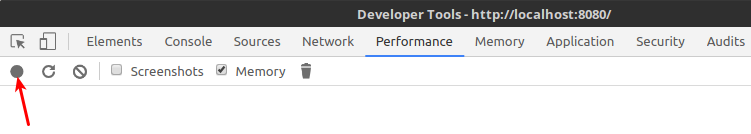
\includegraphics[width=\textwidth]{chrome-devtools-performance-recording-runtime.png}
	\caption{Nagrywanie danych w trakcie działania aplikacji}
\end{figure} 

\begin{figure}[ht]
  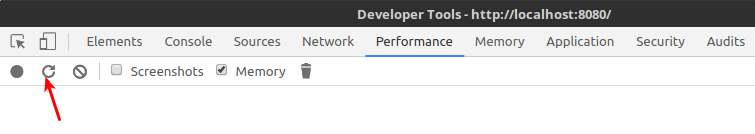
\includegraphics[width=\textwidth]{chrome-devtools-performance-recording-reload.png}
	\caption{Nagrywanie danych od momentu wczytywania strony}
\end{figure}

Po zatrzymaniu nagrywania narzędzie automatycznie dokona reprezentacji zebranych danych za pomocą kilku widoków.

\subsubsection{Widok zbiorczy}

Najwyżej położonym widokiem służacym przedstwieniu zebranych danych jest widok zbiorczy, który składa się z kilku wykresów. Częścią wspólną wszystkich wykresów jest pozioma oś reprezentująca upływający czas. Poniżej opisane zostały wszystkie wykresy wchodzące w skład widoku zbiorczego:

\begin{enumerate}
  \item FPS - wykres ten przedstawia ilość klatek na sekundę, które przeglądarka była w stanie przygotować do wyświetlenia
  \item CPU - wykres ten przedstawia zmieniające sięw  czasie zużycie procesora
  \item NET - wykres przedstawia czas, w którym przeglądarka pobierała wszystkie zasoby potrzebne do wyświetlenia strony oraz czekała na rozwiązanie wszelkich żądań \emph{HTTP} poprzez sieć
  \item HEAP - wykres przestawiający ilość pamięci zajmowanej przez stertę. Bardzo dobrze widać na nim cykliczne działanie zbieracza nieużytków (ang. \emph{Garbage collector}), który jest jedną z metod automatycznego zarządzania dynamicznie przydzieloną pamięcią. Nagłe usuwanie ze sterty niepotrzebnych obiektów powoduje spadek na wykresie i powstawanie charakterystycznych "ząbków".
\end{enumerate}

\begin{figure}[ht]
  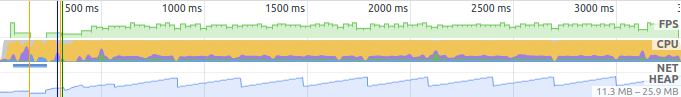
\includegraphics[width=\textwidth]{chrome-devtools-performance-summary-view.png}
	\caption{Przykładowy wygenerowany wykres zbiorczy}
\end{figure}

\subsubsection{Widok sieci}

Widok sieci jest widokiem przedstawiającym w bardziej precyzyjny sposób odcinki czasu, w których ładowane były poszczególne zasoby.

\begin{figure}[ht]
  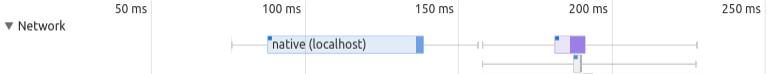
\includegraphics[width=\textwidth]{chrome-devtools-performance-network-view.png}
	\caption{Przykładowy wygenerowany widok sieci}
\end{figure}

\subsubsection{Widok klatek}

Widok klatek jest bardzo małym wykresem przedstawiającym jak zmieniała się liczba klatek na sekundę.

\begin{figure}[ht]
  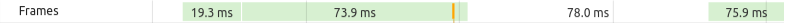
\includegraphics[width=\textwidth]{chrome-devtools-performance-frames-view.png}
	\caption{Przykładowy wygenerowany widok głównego wątku}
\end{figure}

\subsubsection{Widok głównego wątku}

Widok głównego wątku pokazuje dokładnie jakie zadania były wykonywane przez główny wątek. Zadania te pogrupowane są w kategorie za pomocą kolorów:

\begin{enumerate}
  \item niebieski - obejmuje wszystkie zadania związane z ładowaniem zasobów (w tym parsowanie)
  \item żółty - obejmuje wszystkie zadania związane ze skrytami napisanymi w języku \emph{JavaScript}
  \item fioletowy - obejmuje wszystkie zadania związane z renderowaniem
  \item zielony - obejmuje wszystkie zadanie związane z malowaniem
  \item szary - obejmuje wszystkie pozostałe zadanie nie wpasowujące się w pozostałe kategorie
  \item biały - przedstawia okres bezczynności, w którym nie były wykonywane żadne zadania
\end{enumerate}

Przyjęta kolorystyka jest spójna dla wszystkich widoków zakładki \emph{Wydajność}. Po wskazaniu kursorem myszki dowolnego elementu wyświetlone zostają bardziej szczegółowe informacje takie jak np. dokładny czas trwania zadania i jego źródło.

\begin{figure}[ht]
  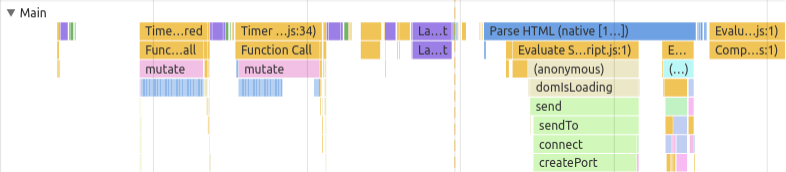
\includegraphics[width=\textwidth]{chrome-devtools-performance-main-view.png}
	\caption{Przykładowy wygenerowany widok klatek}
\end{figure}

\subsection{Badania wydajności pamięciowej}

\subsubsection{Zbieranie danych}

Do zbierania danych na temat wydajności pamięciowej wykorzystany został dokładnie ten sam mechanizm jaki został wykorzystany przy zbieraniu danych na temat wydajości czasowej opisany w rozdziale \cite{gathering-time-performance-data}. Za pomocą tego funkcjonalności możemy włączyć opcję zbierania informacji na temat zużycia pamięci, spowoduje to dodatkowo wyświetlenie widoku wykorzystania pamięci.

\begin{figure}[ht]
  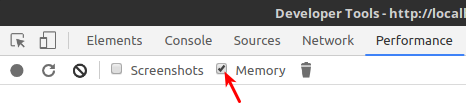
\includegraphics[width=\textwidth]{chrome-devtools-performance-memory-checkbox.png}
	\caption{Włączanie zbierania informacji na temat wykorzystania pamięci}
\end{figure}

\subsubsection{Widok wykorzystania pamięci}

Widok przedstawia jak w czasie zmienia się ilość pamięci zajętej przez stertę. Dodatkowo przedstawia on najmniejszą i najwięszką liczbę elementów w następujących kategoriach:

\begin{enumerate}
  \item Dokumenty (ang. \emph{Documents})
  \item Węzły (ang. \emph{Nodes})
  \item Funkcje nasłuchujące (ang. \emph{Listeners})
  \item Pamięc GPU (ang. \emph{GPU Memory})
\end{enumerate}

\begin{figure}[ht]
  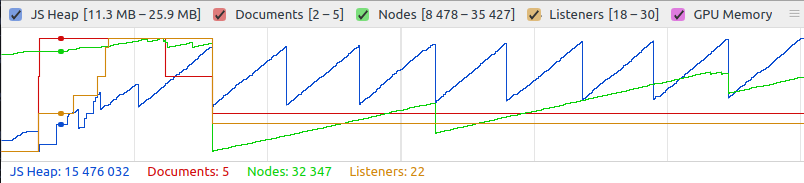
\includegraphics[width=\textwidth]{chrome-devtools-performance-memory-view.png}
	\caption{Przykładowy wygenerowany widok wykorzystania pamięci}
\end{figure}

\subsubsection{Zakładka \emph{Pamięć}}

\emph{Chrome DevTools} udostępnia specjalnie dedykowaną zakładkę o nazwie \emph{Pamięc}, która oferuje dodatkowe funkcjonalności przydatne przy np. debugowaniu aplikacji w celu znalezienia fragmentów kodu odpowiedzialnych za wyciek pamięci. Dostępne opcje to:

\begin{enumerate}
  \item migawka zawartości sterty - pozwala utrwalić aktualny stan sterty, a następnie dokonać przeglądu jej zawartości za pomocą wbudowanej przeglądarki
  \item nagranie profilu alokacji pamięci - pozwala zbierać dane na temat alokacji pamięci z poziomu kodu napisanego w języku \emph{JavaScript}. Dane te można przejrzeć za pomocą trzech widoków. Wykresu, drzewa "od-dołu" (ang. \emph{Bottom Up}) oraz drzewa "od-góry" (ang. \emph{Top Down})
  \item alokacja pamięci przedstawiona na wykresie czasowym - pozwala zbierać dane na temat alokacji pamięci lecz przedstawia je na osi czasowej
\end{enumerate}

Wszystkie opcje umożliwiają opcjonalne zapisanie zebranych danych do pliku na dysku.

\begin{figure}[ht]
  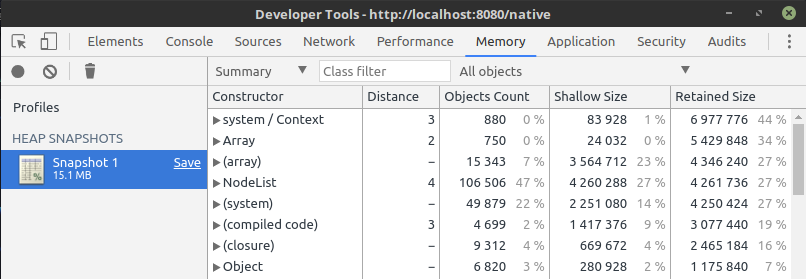
\includegraphics[width=\textwidth]{chrome-devtools-performance-heap-snapshot.png}
	\caption{Przeglądarka zawartości utworzonej migawki sterty}
\end{figure}

\begin{figure}[ht]
  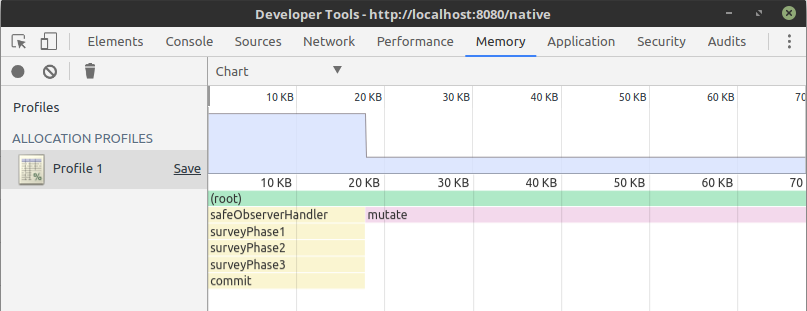
\includegraphics[width=\textwidth]{chrome-devtools-performance-allocation-profile.png}
	\caption{Wykres wygenerowany na podstawie profilu alokacji pamięci}
\end{figure}

\begin{figure}[ht]
  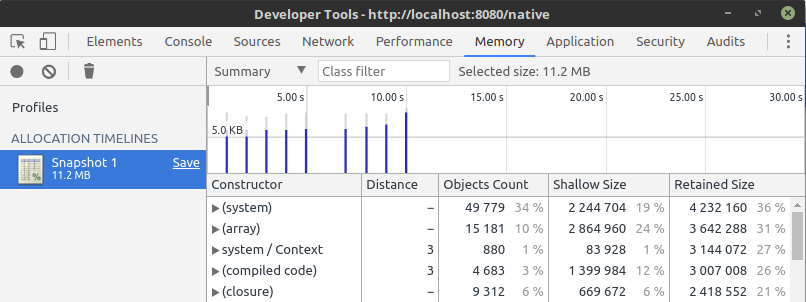
\includegraphics[width=\textwidth]{chrome-devtools-performance-allocation-timeline.png}
	\caption{Wykres czasowy alokacji pamięci}
\end{figure}

\subsubsection{Trace Event Format} \label{trace-event-format-section}

Dane zebrane przez Chrome DevTools w trakcie testów wydajnościowych można zapisać na dysku w formacie o nazwie \emph{Trace Event Format} \cite{trace-event-format}. Dzięki temu możemy dokonać właśnej analizy lub wizualizacji danych. Struktura \emph{Trace Event Format} zgodna jest ze standardem przechowywania danych JSON (ang. \emph{JavaScript Object Notation}) \cite{json} i może występować w dwóch wariantach.

\subsubsection{Wariant tablicowy}
Wariant tablicowy (ang. \emph{JSON Array Format}) - cały plik składa się z tablicy przechowującej obiektu zarejestrowanych zdarzeń. Zdarzenia te nie muszą być poukładane chronologicznie według znaczników czasu. 

\begin{lstlisting}[caption=Przykładowy wariant tablicowy]
[{
  "name": "Asub",
  "cat": "PERF",
  "ph": "B",
  "pid": 22630,
  "tid": 22630,
  "ts": 829
}, {
  "name": "Asub",
  "cat": "PERF",
  "ph": "E",
  "pid": 22630,
  "tid": 22630,
  "ts": 833
}]
\end{lstlisting}

\subsubsection{Wariant obiektowy}

Wariant obiektowy (ang. \emph{JSON Object Format}) - bardziej elsatyczny format, w którym plik składa się z jednego, głównego obiektu. Obiekt ten może posiadać następujące pola:

\begin{enumerate}
  \item traceEvents - jedyne wymagane pole, które jest tablicą zarejestrowanych zdarzeń odpowiadająca dokładnie wariantowi tablicowemu formatu \emph{Trace Event Format}
  \item displayTimeUnit - jednostka, w której podane zostały znaczniki czasu. Dostępne jednostki to \emph{ms} oraz \emph{ns}. Domyślna jednostka to \emph{ms}
  \item systemTraceEvents - ciąg znaków kompatybilnych z \emph{Linux ftrace} lub \emph{Windows ETW}
  \item powerTraceAsString - ciąg znaków kompatybilnych z \emph{BattOr}
  \item stackFrames - struktura przechowująca informacje o ramkach odłożonych na stosie
  \item samples - tablica przechowująca dane rozszerzające traceEvents o informacje zarejestrowane na poziomie systemu operacyjnego 
\end{enumerate}

Dopuszcza się możliwość definicji pól o nazwach innych niż wymienione wcześniej dla dodatkowego opisania danych (metadane)

\begin{lstlisting}[caption=Przykładowy wariant obiektowy]
{
  "traceEvents": [[{
    "name": "Asub",
    "cat": "PERF",
    "ph": "B",
    "pid": 22630,
    "tid": 22630,
    "ts": 829
  }, {
    "name": "Asub",
    "cat": "PERF",
    "ph": "E",
    "pid": 22630,
    "tid": 22630,
    "ts": 833
  }],
  "displayTimeUnit": "ns",
}
\end{lstlisting}

\subsubsection{Zdarzenia}

Podstawowymi obiektami, które można poddać analizie są zdarzenia. Istnieje kilka rodzajów zdarzeń. Poniżej przedstawiono pola występujące w każdym zdarzeniu niezależnie od jego typu:

\begin{enumerate}
  \item name - nazwa zdarzenia
  \item cat - kolekcja oddzielonych przecinkiem kategorii powiązanych ze zdarzeniem
  \item ph - pojedynczy znak określający typ zdarzenia. Table prawidłowych wartości została przedstawiona poniżej.
  \item ts - znacznik czasowy zdarzenia podany z dokładnością do milisekundy
  \item tts - opcjonalny znacznik czasowy wątku zdarzenia podany z dokładnością do milisekundy
  \item pid - identyfikator procesu, który spowodował zaistnienie zdarzenia
  \item tid - identyfikator wątku, który spowodował zaistnienie zdarzenia
  \item args - argumenty, które zostały dostarczone dla zdarzenia
\end{enumerate}

\begin{center}
  \begin{tabularx}{\textwidth}{|X|X|}\hline
    \emph{Typ zdarzenia} & \emph{Fazy zdarzenia}\\ \hline
    Zdarzenia trwające (\emph{ang. duration events}) & \textbf{B} początek (\emph{ang. begin}),\newline
    \textbf{E} koniec (\emph{ang. end})\\ \hline
    Zdarzenia kompletne (\emph{ang. complete events}) & \textbf{X}\\ \hline
    Zdarzenia natychmiastowe (\emph{ang. instant events}) & \textbf{i, I}(przestarzałe)\\ \hline
    Zdarzenia zliczające (\emph{ang. counter events}) & \textbf{c}\\ \hline
    Zdarzenia asynchroniczne (\emph{ang. async events}) & \textbf{b} (początek),\newline
    \textbf{n} (natychmiastowe zdarzenie asynchroniczne),\newline
    \textbf{e} (koniec)\newline\newline
    \textit{Przestarzałe}\newline
    \textbf{S} (początek),\newline
    \textbf{T} (krok kolejny),\newline
    \textbf{p} (krok poprzedni),\newline
    \textbf{F} (koniec)\\ \hline
    Zdarzenia przepływające (\emph{ang. flow events}) & \textbf{s} (początek),\newline
    \textbf{t} (krok),\newline
    \textbf{f} (koniec)\\ \hline
    Zdarzenia obiektowe (\emph{ang. object events}) & \textbf{N} (stworzenie)\newline
    \textbf{O} (migawka)\newline
    \textbf{D} (zniszczenie)\\ \hline
    Zdarzenia z metadanymi (\emph{ang. metadata events}) & \textbf{M}\\ \hline
    Zdarzenia zrzutu pamięci (\emph{ang. memory dump events}) & \textbf{V} (zrzut pamięci globalnej)\newline
    \textbf{v} (zrzut pamięci procesu)\\ \hline
    Zdarzenia synchronizacji zegara (\emph{ang. clock sync events}) & \textbf{c}\\ \hline
    Zdarzenia kontekstowe (\emph{ang. context events}) & \textbf{(, )}\\ \hline
  \end{tabularx}
\end{center}

Poniżej przedstawiono opis każdego z możliwych typów zdarzeń:

\begin{enumerate}
  \item zdarzenia trwające - umożliwiają określenie czasu trwania pracy nad danym wątkiem. Zdarzenia czasowe są określane przez typy \textbf{B} i \textbf{E}. Zdarzenie \textbf{B} musi nastąpić przed odpowiednim wydarzeniem \textbf{E}. Można zagnieżdżać zdarzenia \textbf{B} i \textbf{E}. Znaczniki czasowe dla zdarzeń muszą być ułożone w kolejności rosnącej dla danego wątku. Znaczniki czasu w różnych wątkach nie muszą być ułożone w kolejności rosnącej.
  \item zdarzenia kompletne - każde kompletne zdarzenie logicznie łączy parę zdarzeń (\textbf{B} i \textbf{E}). Kompletne zdarzenia są oznaczone przez typ fazy \textbf{X}.
  \item zdarzenia natychmiastowe - odpowiadają czemuś co miało miejsce lecz bez przypisanego czasu trwania.
  \item zdarzenia zliczające - mogą śledzić wartość lub wiele wartości zmieniających się w czasie.
  \item zdarzenia asynchroniczne - służą do rejestrowania asynchronicznych operacji. Mogą pochodzić zarówno z różnych procesów jak i wątków.
  \item zdarzenia przepływające - z założenia są bardzo podobne do zdarzeń asynchronicznych, ale dodatkowo pozwalają na łączenie ich ze sobą w wątkach i/lub procesach.
  \item zdarzenia obiektowe - służą za konstrukcję do śledzenia złożonych struktur danych.
  \item zdarzenia z metadanymi - są używane do powiązania dodatkowych informacji z wydarzeniami.
  \item zdarzenia zrzutu pamięci - odpowiadają zrzutom pamięci procesu lub grupie procesów.
  \item zdarzenia synchronizacji zegara - służą do synchonizacji czasu w przypadku gdy zdarzenia rejestrowane są przez różne byty.
  \item zdarzenia kontekstowe - są używane do oznaczania sekwencji zdarzeń.
\end{enumerate}

\begin{lstlisting}[caption=Przykładowe zdarzenie]
{
  "name": "myName",
  "cat": "category,list",
  "ph": "B",
  "ts": 12345,
  "pid": 123,
  "tid": 456,
  "args": {
    "someArg": 1,
    "anotherArg": {
      "value": "my value"
    }
  }
\end{lstlisting}

\section{Aplikacje wspomające pomiary} \label{utils}

W ramach pisania pracy magisterskiej zostały napisane trzy mniejsze aplikacje, które w znaczący sposób pomogły zebrać potrzebne dane. Głównym celem była automatyzacja wszystkich czasochłonnych i żmudnych czynności. Osiągając cel główny udało się również zminimalizować efekt zniekształcenia pomiarów poprzez manualną ingerencję człowieka.

\subsection{javascript-frameworks-benchmark}

\subsubsection{Opis}

\emph{javascript-frameworks-benchmark} to aplikacja, która przechowuje kod źródłowy wszystkich implementacji opartych na opisanych w pracy magisterskiej bibliotekach programistycznych. Po jej uruchomieniu pod lokalnym adresem \emph{http://localhost} i domyślnym porcie \emph{8080} dostępna jest strona za pomocą, której w łatwy sposób można przejść do wybranej przez siebie implementacji.

\begin{figure}[ht]
  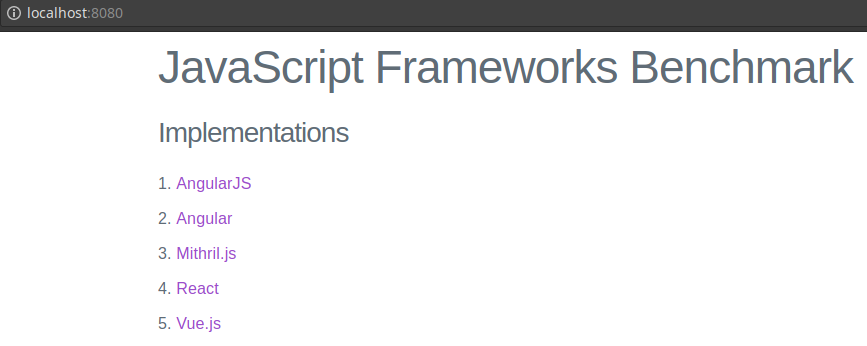
\includegraphics[width=\textwidth]{javascript-frameworks-benchmark.png}
	\caption{Widok strony wyboru implementacji}
\end{figure}

\subsubsection{Specyfikacja wewnętrzna}

Aplikacja została napisana w języku \emph{JavaScript} w standardzie ECMAScript 2016 \cite{es2016}. Środowiskiem uruchomieniowym jest \emph{Node.js} \cite{node.js} w wersji \emph{8.1.4}. Do poprawnego zainstalowania zewnętrznych zależności potrzebny jest menedżer pakietów \emph{Yarn} \cite{yarn}. Serwer obsługujący żadania \emph{HTTP} oparty został na bibliotece \emph{Express} \cite{express}.

\subsubsection{Specyfikacja zewnętrzna}

\textbf{Sposób uruchomienia programu} \newline

Żeby uruchomić program należy przejść za pomocą konsoli do głównego folderu programu a następnie wywołać następujące komendy:

\begin{lstlisting}
yarn install
yarn start
\end{lstlisting}

\textbf{Format danych wejściowych} \newline

Aplikacja nie przyjmuje danych wejściowych. \newline

\textbf{Format danych wyjściowych} \newline

Aplikacja nie podaje żadnych danych na wyjściu. Odpowiada na żądania \emph{HTTP} pod domyślnym adresem \emph{http://localhost:8080}

\subsection{chrome-performance-logs-recorder}

\subsubsection{Opis}

\emph{chrome-performance-logs-recorder} to aplikacja, która w automatyczny sposób uruchamia przeglądarkę internetową, przechodzi pod określony adres a następnie zbiera informacje związane z wydajnością aby pod koniec zapisać je do pliku w formacie \emph{JSON}. 

\subsubsection{Specyfikacja wewnętrzna}

Aplikacja została napisana w języku \emph{JavaScript} w standardzie ECMAScript 2016 \cite{es2016}. Środowiskiem uruchomieniowym jest \emph{Node.js} \cite{node.js} w wersji \emph{8.1.4}. Do poprawnego zainstalowania zewnętrznych zależności potrzebny jest menedżer pakietów \emph{Yarn} \cite{yarn} oraz przeglądarka internetowa \emph{Chrome}.

Automatyczne działanie opiera się na uruchomieniu serwera \emph{Selenium} \cite{selenium}, który to uruchamia a następnie podłącza się do przeglądarki internetowej sam udostępniajać interfejs programistyczny do większości akcji, które może robić standardowy użytkownik przeglądarki. Aby korzystać w pełni z funkcjonalności oferowanych przez \emph{Selenium} użyto wiązań (ang. \emph{bindings}) dostarczanych przez paczkę \emph{wd} \cite{wd}, które pozwalają na dostęp do interfejsu \emph{Selenium} z poziomu języka \emph{JavaScript} w środowisku \emph{Node.js}.

\subsubsection{Specyfikacja zewnętrzna}

\textbf{Sposób uruchomienia programu} \newline

Żeby uruchomić program należy przejść za pomocą konsoli do głównego folderu programu a następnie wywołać następujące komendy:

\begin{lstlisting}
yarn install
yarn ./build/main.js [parametry]
\end{lstlisting}

\textbf{Format danych wejściowych} \newline

Aplikacja przyjmuje następujące parametry:

\begin{itemize}
  \item \emph{-{}-debug} (domyślna wartość \emph{false}) - flaga włączająca dodatkowe infomacje na wyjściu
  \item \emph{-{}-duration} (domyślna wartość \emph{5000}) - czas zbierania informacji podanych w milisekundach
  \item \emph{-{}-filter-event-names} (domyślna wartość \emph{' '}) - odseprowane przecinkami nazwy zdarzeń, o których informacje mają być zbierane przez aplikację
  \item \emph{-{}-local-storage} (domyślna wartość \emph{key:value}) - pozwala zapisać w przeglądarce jedną parę klucz-wartość za pomocą mechanizmu przeglądarki \emph{LocalStorage}
  \item \emph{-{}-output-filename} (domyślna wartość \emph{'trace.json}) - nazwa pliku do którego mają zostać zapisane informacje
  \item \emph{-{}-silent} (domyślna wartość \emph{false}) - flaga wyłączająca wszelkie informacje na wyjściu
  \item \emph{-{}-trace-categories} (domyślna wartość \emph{'devtools.timeline,} \newline \emph{disabled-by-default-devtools.timeline.frame,rail'}) - odseparowane przecinkami kategorie zdarzeń, o których informacje mają być zbierane przez aplikację
  \item \emph{-{}-trim} (domyślna wartość \emph{0}) - podana w procentach ilość zdarzeń, która ma zostać obcięta z końcowego raportu (na początku oraz na końcu)
  \item \emph{-{}-url} (domyślna wartość \emph{' '}) - adres strony internetowej, na podstawie której mają być zbierane przez aplikację informacje
  \item \emph{-{}-verbose} (domyślna wartość \emph{false}) - flaga włączająca dodatkowe informacje na wyjściu
\end{itemize}

\textbf{Format danych wyjściowych} \newline

Dane wyjściowe zapisane do pliku o rozszerzeniu \emph{JSON} są zgodne z opisanym wcześniej formatem \emph{Trace Event Format} \ref{trace-event-format-section}.

\subsection{trace-event-format-analyzer}

\subsubsection{Opis}

\emph{trace-event-format-analyzer} to aplikacja, która potrafi dokonać analizy setki megabajtów danych zarejestrowanych w formacie \emph{Trace Event Format}.

\subsubsection{Specyfikacja wewnętrzna}

Aplikacja została napisana w języku \emph{JavaScript} w standardzie ECMAScript 2016 \cite{es2016}. Środowiskiem uruchomieniowym jest \emph{Node.js} \cite{node.js} w wersji \emph{8.1.4}. Do poprawnego zainstalowania zewnętrznych zależności potrzebny jest menedżer pakietów \emph{Yarn} \cite{yarn}.

Aplikacja wczytuje plik z rozszerzeniem \emph{JSON} a następnie iteruje po kolekcji zdarzeń dokonując odpowiednich obliczeń.

\subsubsection{Specyfikacja zewnętrzna}

\textbf{Sposób uruchomienia programu} \newline

Żeby uruchomić program należy przejść za pomocą konsoli do głównego folderu programu a następnie wywołać następujące komendy:

\begin{lstlisting}
yarn install
yarn ./build/main.js [parametry]
\end{lstlisting}

\textbf{Format danych wejściowych} \newline

Aplikacja przyjmuje następujące parametry:

\begin{itemize}
  \item \emph{-{}-complete-events} (domyślna wartość \emph{' '}) - odseparowane przecinkami nazwy zdarzeń kompletnych, które mają zostać poddane analizie
  \item \emph{-{}-decimal-places} (domyślna wartość \emph{4}) - liczba miejsc po przecinku, do których mają zostać zaokrąglone wyniki
  \item \emph{-{}-duration-events} (domyślna wartość \emph{' '}) - odseparowane przecinkami nazwy zdarzeń trwających, które mają zostać poddane analizie
  \item \emph{-{}-immediate-events} (domyślna wartość \emph{' '}) - odseparowane przecinkami nazwy zdarzeń natychmiastowych, które mają zostać poddane analizie
  \item \emph{-{}-output} (domyślna wartość \emph{'false}) - flaga włączająca zapis analizy do pliku w formacie \emph{JSON}
  \item \emph{-{}-paths} (domyślna wartość \emph{' '}) - odseparowane przecinkami ścieżki plików, które mają zostać wczytane oraz poddane analizie
  \item \emph{-{}-silent} (domyślna wartość \emph{false}) - flaga wyłączająca wszelkie informacje na wyjściu
  \item \emph{-{}-verbose} (domyślna wartość \emph{false}) - flaga włączająca dodatkowe informacje na wyjściu
\end{itemize}

\textbf{Format danych wyjściowych} \newline

Dane wyjściowe, które opcjonalnie mogą zostać zapisane do pliku o rozszerzeniu \emph{JSON} są obiektem o następujących właściwościach:

\begin{enumerate}
  \item \emph{completeEvents} - obiekt zdarzeń kompletnych, którego właściwości odpowiadają nazwom analizowanych zdarzeń tego typu
  \item \emph{durationEvents} - obiekt zdarzeń trwających, którego właściwości odpowiadają nazwom analizowanych zdarzeń tego typu
  \item \emph{immediateEvents} - obiekt zdarzeń natychmiastowych, którego właściwości odpowiadają nazwom analizowanych zdarzeń tego typu
\end{enumerate}

Każdy obiekt odpowiadający konkretnemu zdarzeniu posiada następujące właściwości:

\begin{enumerate}
  \item \emph{deltas} - przechowuje wyliczone statystyki na podstawie czasu pomiędzy kolejnymi zdarzeniami (jednostka to milisekundy)
  \item \emph{eps} - przechowuje wyliczone statystyki na podstawie ilości zdarzeń na sekundę (jednostka to zdarzenia na sekundę)
\end{enumerate}

Obiekt przechowujący wyliczone statystyki posiada następujace właściwości:

\begin{enumerate}
  \item \emph{min} - minimalna zarejestrowana wartość
  \item \emph{mean} - średnia zarejestrowanych wartości
  \item \emph{percentiles} - obliczone percentyle kolejno 50\%, 66\%, 75\%, 80\%, 85\%, 90\%, 95\%, 98\%, 99\%, 100\%
  \item \emph{standardDeviation} - odchylenie standardowe
  \item \emph{variance} - wariancja
\end{enumerate}

\section{Porównanie wyników i wnioski}

\section{Podsumowanie}

\subsection{Dalszy rozwój}

\begin{thebibliography}{11}
  \bibitem{milligram}
    \url{http://milligram.io/}
  \bibitem{node.js}
    \url{http://nodejs.org/}
  \bibitem{v8}
    \url{https://github.com/v8/v8}
  \bibitem{npm}
    \url{https://www.npmjs.com/}
  \bibitem{yarn}
    \url{https://yarnpkg.com/}
  \bibitem{es2016}
    \url{https://www.ecma-international.org/ecma-262/7.0/}
  \bibitem{express}
    \url{https://expressjs.com/}
  \bibitem{selenium}
    \url{https://github.com/SeleniumHQ/selenium}
  \bibitem{wd}
    \url{https://github.com/admc/wd}
  \bibitem{spdy}
    \url{http://dev.chromium.org/spdy/}
  \bibitem{w3c}
    \url{https://www.w3.org/}
  \bibitem{w3c-rec-html51}
    \url{https://www.w3.org/TR/html51/}
  \bibitem{w3c-rec-css3-background}
    \url{https://www.w3.org/TR/css3-background/}
  \bibitem{w3c-rec-css3-box}
    \url{https://www.w3.org/TR/css3-box/}
  \bibitem{w3c-rec-css3-cascade}
    \url{https://www.w3.org/TR/css-cascade-3/}
  \bibitem{w3c-rec-css3-color}
    \url{https://www.w3.org/TR/css3-color/}
  \bibitem{w3c-rec-css3-content}
    \url{https://www.w3.org/TR/css-content-3/}
  \bibitem{w3c-rec-css3-fonts}
    \url{https://www.w3.org/TR/css-fonts-3/}
  \bibitem{w3c-rec-css3-gcpm}
    \url{https://www.w3.org/TR/css-gcpm-3/}
  \bibitem{w3c-rec-css3-template}
    \url{https://www.w3.org/TR/css-template-3/}
  \bibitem{w3c-rec-css3-mediaqueries}
    \url{https://www.w3.org/TR/css3-mediaqueries/}
  \bibitem{w3c-rec-css3-multicol}
    \url{https://www.w3.org/TR/css3-multicol/}
  \bibitem{w3c-rec-css3-page}
    \url{https://www.w3.org/TR/css3-page/}
  \bibitem{w3c-rec-css3-selectors}
    \url{https://www.w3.org/TR/css3-selectors/}
  \bibitem{w3c-rec-css3-ui}
    \url{https://www.w3.org/TR/css-ui-3/}
  \bibitem{w3c-rec-dom-level-1}
    \url{https://www.w3.org/TR/DOM-Level-1/}
  \bibitem{w3c-rec-dom-level-2}
    \url{https://www.w3.org/TR/DOM-Level-2/}
  \bibitem{w3c-rec-dom-level-3-core}
    \url{https://www.w3.org/TR/DOM-Level-3-Core/}
  \bibitem{w3c-rec-dom-level-3-ls}
    \url{https://www.w3.org/TR/DOM-Level-3-LS/}
  \bibitem{w3c-rec-dom-level-3-xpath}
    \url{https://www.w3.org/TR/DOM-Level-3-XPath/}
  \bibitem{w3c-rec-dom-level-3-views}
    \url{https://www.w3.org/TR/DOM-Level-3-Views/}
  \bibitem{w3c-rec-dom-level-3-requirements}
    \url{https://www.w3.org/TR/DOM-Requirements/}
  \bibitem{w3c-rec-dom-level-3-val}
    \url{https://www.w3.org/TR/DOM-Level-3-Val/}
  \bibitem{rfc2616}
    \url{https://www.ietf.org/rfc/rfc2616}
  \bibitem{rfc2660}
    \url{https://www.ietf.org/rfc/rfc2660}
  \bibitem{rfc7540}
    \url{https://www.ietf.org/rfc/rfc7540}
  \bibitem{chrome}
    \url{https://www.google.pl/chrome/browser/desktop/index.html}
  \bibitem{chrome-devtools}
    \url{https://developers.google.com/web/tools/chrome-devtools/}
  \bibitem{trace-event-format}
    \url{https://docs.google.com/document/d/1CvAClvFfyA5R-PhYUmn5OOQtYMH4h6I0nSsKchNAySU/edit}
  \bibitem{json}
    \url{http://www.json.org/}
\end{thebibliography}

\end{document}
